\documentclass[12pt,a4paper]{article}
\usepackage[margin=2.2cm]{geometry}
\usepackage[T1]{fontenc}
\usepackage{mathpazo}
\usepackage{amsmath,amssymb}
\usepackage{tikz}
\usepackage{enumitem}
\usepackage{needspace}
\raggedbottom
\setlength{\parindent}{0pt}
\setlength{\parskip}{7pt}
\setlist{itemsep=0pt,topsep=2pt}
\pagestyle{plain}
\newcommand{\Ahat}{\hat A}
\newcommand{\R}{\mathbb{R}}
\newcommand{\h}[1]{\par\needspace{6\baselineskip}\medskip\textbf{\large #1}\par}

\begin{document}

\begin{center}
{\Large\bfseries Vanilla GCN: Mathematical Modelling}\\[4pt]
[Your name] \quad [Roll no.]
\end{center}
Detecting illicit Bitcoin transactions on the Elliptic dataset using a 2-layer Vanilla GCN.

%==============================================================
\h{1. Graph Representation}
\[
  G = (V, E), \quad |V| = 203{,}769 \ (\text{transactions}), \quad |E| = 234{,}355 \ (\text{money flows})
\]
Adjacency matrix $A \in \{0,1\}^{N\times N}$, \ feature matrix $X \in \R^{N\times F}$ ($F = 165$), \
label $y \in \{0, 1\}$ ($0$ = licit, $1$ = illicit).

\h{2. Symmetric Normalisation}
\[
  \tilde A = A + I_N, \qquad \tilde D_{ii} = \sum_j \tilde A_{ij}, \qquad \Ahat = \tilde D^{-1/2}\,\tilde A\,\tilde D^{-1/2}
\]
Self-loops let a node keep its own features. Normalisation gives a fair weighted average, so high-degree nodes do not dominate.

Feature normalisation: \ $x_{ij} \leftarrow \dfrac{x_{ij} - \mu_j}{\sigma_j}$ \ (mean $\mu_j$, standard deviation $\sigma_j$ of feature $j$).

\h{3. GCN Layer and Forward Pass}
\[
  H^{(l+1)} = \sigma\big(\Ahat\, H^{(l)}\, W^{(l)}\big)
\]
$H^{(l)}$ = node features at layer $l$, \ $W^{(l)}$ = learnable weights, \ $\Ahat$ = normalised adjacency,
\ $\sigma$ = ReLU.
\[
  Z = \mathrm{softmax}\Big(\Ahat\cdot \mathrm{ReLU}\big(\Ahat\cdot X\cdot W^{(0)}\big)\cdot W^{(1)}\Big)
\]
$N = 203{,}769$, \ $F = 165$, \ $H = 100$ hidden, \ $C = 2$ classes:
\quad $X \rightarrow N\times F$, \quad $H^{(1)} \rightarrow N\times H$, \quad $Z \rightarrow N\times C$

\h{4. Loss Function}
Weighted cross-entropy over labelled training nodes only (illicit is rare, so $w_1 = 0.7$, $w_0 = 0.3$):
\[
  \mathcal L = -\frac{1}{\sum_i w_{y_i}} \sum_{i\in V_{\text{train}}} w_{y_i}\, \log Z_{i, y_i}
\]

\h{5. Training}
Minimise $\mathcal L$ over $\theta = \{W^{(0)}, W^{(1)}\}$ with Adam: \
$\theta \leftarrow \theta - \eta\cdot\text{Adam}(\nabla_\theta\mathcal L)$, \ $\eta = 0.01$, 200 epochs.

One epoch: forward pass $\rightarrow$ loss on train nodes $\rightarrow$ backpropagation $\rightarrow$ update weights.
Train on time steps 1--34, test on 35--49.

\h{6. Evaluation Metrics}
\[
  \text{Precision} = \frac{TP}{TP + FP}, \qquad \text{Recall} = \frac{TP}{TP + FN}, \qquad
  F_1 = \frac{2\cdot P\cdot R}{P + R}
\]
Our result ($TP = 507$, $FP = 182$, $FN = 576$): \
Precision $= \frac{507}{689} = 0.736$, \ Recall $= \frac{507}{1083} = 0.468$, \ $F_1 = 0.572$.

%==============================================================
\h{7. Worked Example: Graph}
Five transactions, $V = \{0,1,2,3,4\}$, \ $E = \{(0,1), (1,2), (1,3), (2,3), (3,4)\}$.

\begin{center}
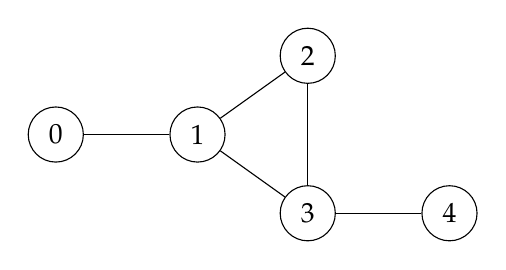
\begin{tikzpicture}[every node/.style={circle, draw, minimum size=7mm}]
  \node (0) at (0,0) {0}; \node (1) at (1.8,0) {1}; \node (2) at (3.2,1) {2};
  \node (3) at (3.2,-1) {3}; \node (4) at (5,-1) {4};
  \draw (0)--(1); \draw (1)--(2); \draw (1)--(3); \draw (2)--(3); \draw (3)--(4);
\end{tikzpicture}
\end{center}
\[
  A = \begin{bmatrix}
  0&1&0&0&0\\ 1&0&1&1&0\\ 0&1&0&1&0\\ 0&1&1&0&1\\ 0&0&0&1&0
  \end{bmatrix}, \quad d = [1,3,2,3,1], \quad D = \mathrm{diag}(1,3,2,3,1)
\]
Add self-loops:
\[
  \tilde A = A + I = \begin{bmatrix}
  1&1&0&0&0\\ 1&1&1&1&0\\ 0&1&1&1&0\\ 0&1&1&1&1\\ 0&0&0&1&1
  \end{bmatrix}, \quad \tilde d = [2,4,3,4,2], \quad \tilde D = \mathrm{diag}(2,4,3,4,2)
\]

\h{8. Normalised Adjacency}
\[
  \tilde D^{-1/2} = \mathrm{diag}\Big(\tfrac{1}{\sqrt2},\ \tfrac12,\ \tfrac{1}{\sqrt3},\ \tfrac12,\ \tfrac{1}{\sqrt2}\Big),
  \qquad \Ahat = \tilde D^{-1/2}\tilde A\tilde D^{-1/2}
\]
\[
  \Ahat_{ij} = \frac{\tilde A_{ij}}{\sqrt{\tilde d_i \tilde d_j}}
  \qquad\Rightarrow\qquad
  \Ahat \approx \begin{bmatrix}
  0.5 & 0.354 & 0 & 0 & 0\\
  0.354 & 0.25 & 0.289 & 0.25 & 0\\
  0 & 0.289 & 0.333 & 0.289 & 0\\
  0 & 0.25 & 0.289 & 0.25 & 0.354\\
  0 & 0 & 0 & 0.354 & 0.5
  \end{bmatrix}
\]
e.g.\ $\Ahat_{01} = \frac{1}{\sqrt{2\cdot4}} = \frac{1}{2\sqrt2} \approx 0.354$, \quad
$\Ahat_{12} = \frac{1}{\sqrt{4\cdot3}} = \frac{1}{2\sqrt3} \approx 0.289$.

\h{9. Features and Labels}
$f_1$ = unusual output pattern, \ $f_2$ = normal fee pattern.
\[
  X = \begin{bmatrix} 1&0\\ 1&1\\ 1&0\\ 0&1\\ 0&1 \end{bmatrix}
  \qquad
  \begin{array}{l}
  \text{Node 0: illicit, } y_0 = [0, 1]\\
  \text{Node 4: licit, } y_4 = [1, 0]\\
  \text{Nodes 1, 2, 3: unlabelled}
  \end{array}
\]

\h{10. Layer 1: $H^{(1)} = \mathrm{ReLU}(\Ahat X W^{(0)})$}
Take $W^{(0)} = I$ (only neighbour mixing), so $H^{(1)} = \mathrm{ReLU}(\Ahat X)$:
\begin{align*}
  H^{(1)}_0 &= 0.5(1,0) + 0.354(1,1) = (0.854,\ 0.354)\\
  H^{(1)}_1 &= 0.354(1,0) + 0.25(1,1) + 0.289(1,0) + 0.25(0,1) = (0.892,\ 0.5)\\
  H^{(1)}_2 &= 0.289(1,1) + 0.333(1,0) + 0.289(0,1) = (0.622,\ 0.577)\\
  H^{(1)}_3 &= 0.25(1,1) + 0.289(1,0) + 0.25(0,1) + 0.354(0,1) = (0.539,\ 0.854)\\
  H^{(1)}_4 &= 0.354(0,1) + 0.5(0,1) = (0,\ 0.854)
\end{align*}
All values are $\ge 0$, so ReLU makes no changes:
\[
  H^{(1)} \approx \begin{bmatrix}
  0.854 & 0.354\\ 0.892 & 0.500\\ 0.622 & 0.577\\ 0.539 & 0.854\\ 0 & 0.854
  \end{bmatrix}
\]

\h{11. Layer 2: $Z = \Ahat H^{(1)} W^{(1)}$}
\[
  W^{(1)} = \begin{bmatrix} -1 & 1\\ 1 & -1 \end{bmatrix}, \qquad M = \Ahat H^{(1)}, \qquad Z = M W^{(1)}
\]
\begin{align*}
  M_0 &= 0.5(0.854,\ 0.354) + 0.354(0.892,\ 0.5) = (0.742,\ 0.354) &\Rightarrow\ Z_0 &= (-0.389,\ 0.389)\\
  M_4 &= 0.354(0.539,\ 0.854) + 0.5(0,\ 0.854) = (0.190,\ 0.729) &\Rightarrow\ Z_4 &= (0.538,\ -0.538)
\end{align*}
Same for all rows ($Z_{i0} = M_{i1} - M_{i0}$, \ $Z_{i1} = -Z_{i0}$):
\[
  M \approx \begin{bmatrix}
  0.742 & 0.354\\ 0.839 & 0.630\\ 0.620 & 0.583\\ 0.537 & 0.807\\ 0.190 & 0.729
  \end{bmatrix}
  \qquad
  Z \approx \begin{bmatrix}
  -0.389 & 0.389\\ -0.209 & 0.209\\ -0.037 & 0.037\\ 0.270 & -0.270\\ 0.538 & -0.538
  \end{bmatrix}
\]

\h{12. Softmax}
\[
  P_{ic} = \frac{e^{Z_{ic}}}{\sum_{c'} e^{Z_{ic'}}}
\]
Node 0: \ $P_{0,1} = \dfrac{e^{0.389}}{e^{-0.389} + e^{0.389}} \approx 0.685$
\quad $\Rightarrow P_0 = [0.315,\ 0.685]$ \ $\rightarrow$ illicit $\checkmark$

Node 4: \ $P_{4,0} = \dfrac{e^{0.538}}{e^{0.538} + e^{-0.538}} \approx 0.746$
\quad $\Rightarrow P_4 = [0.746,\ 0.254]$ \ $\rightarrow$ licit $\checkmark$

\[
  P \approx \begin{bmatrix}
  0.315 & 0.685\\ 0.397 & 0.603\\ 0.481 & 0.519\\ 0.632 & 0.368\\ 0.746 & 0.254
  \end{bmatrix}
  \qquad
  \begin{array}{l}
  \text{Node 0: illicit } \checkmark\\ \text{Node 1: illicit (predicted)}\\ \text{Node 2: illicit (borderline)}\\
  \text{Node 3: licit (predicted)}\\ \text{Node 4: licit } \checkmark
  \end{array}
\]
Unlabelled node 1 is flagged illicit because it receives money directly from the illicit node 0.

\h{13. Cross-Entropy Loss}
\[
  \mathcal L = \frac12\big[-\log P_{0,1} - \log P_{4,0}\big] = \frac12\big[-\log 0.685 - \log 0.746\big]
  = \frac{0.378 + 0.293}{2} \approx \underline{\underline{0.336}}
\]

\h{14. Gradient and Update}
\[
  \frac{\partial \mathcal L_i}{\partial Z_{ic}} = P_{ic} - y_{ic}
\]
Node 0: \ $[0.315 - 0,\ 0.685 - 1] = [0.315,\ -0.315]$ \qquad
Node 4: \ $[0.746 - 1,\ 0.254 - 0] = [-0.254,\ 0.254]$
\[
  \frac{\partial\mathcal L}{\partial W^{(1)}} = M^T\,\frac{\partial\mathcal L}{\partial Z} \approx
  \begin{bmatrix} 0.093 & -0.093\\ -0.037 & 0.037 \end{bmatrix},
  \qquad
  W \leftarrow W - \eta\,\frac{\partial\mathcal L}{\partial W}
\]
This completes one training iteration of the Vanilla GCN.

\end{document}
